%! Author = drakanoy
%! Date = 10.09.2024

% Preamble
\documentclass[12pt]{article}

% Packages
\usepackage[utf8]{inputenc}
\usepackage[T2A]{fontenc}
\usepackage[english, russian]{babel}
\usepackage[a4paper, includefoot, left=1.5cm, right=1.5cm, top=1cm, bottom=1.5cm, headsep=1cm, footskip=1cm]{geometry}
\usepackage{makecell}
\usepackage{amsmath}
\usepackage{graphicx}
\usepackage{enumitem}
\usepackage{svg}
\usepackage{multirow}
\usepackage{hyperref}
\usepackage{mathtools}
\usepackage{amssymb}
\usepackage{textcomp}

% Document
\begin{document}
\begin{large}
\begin{center}
\LARGE \textbf{Домашняя работа}
\par
\LARGE \textbf{Кононов Александр Михайлович}
\par
    \textbf{26.10.2024}
\end{center}
\par Условие:
\par
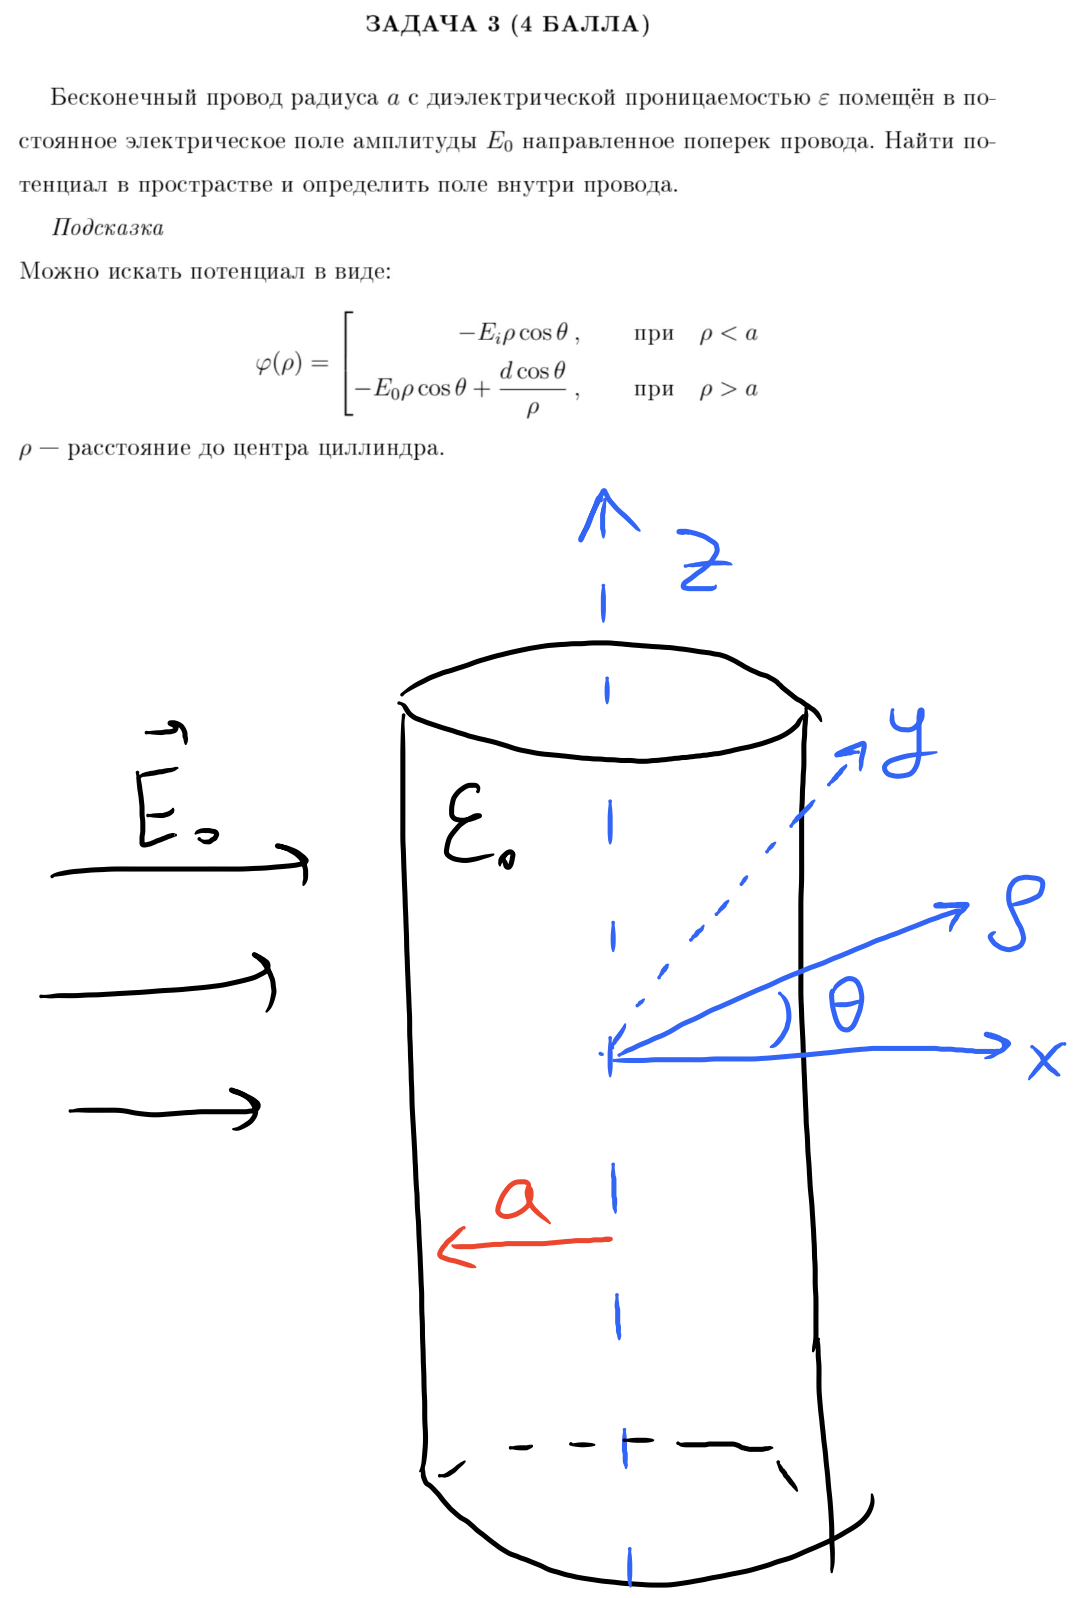
\includegraphics[width=1\textwidth]{photo.png}
%\begin{center}
%\underline{Рисунок 1}:
%\end{center}
\par Решение:
\par Будем считать, что поле направлено по оси z.
\par
%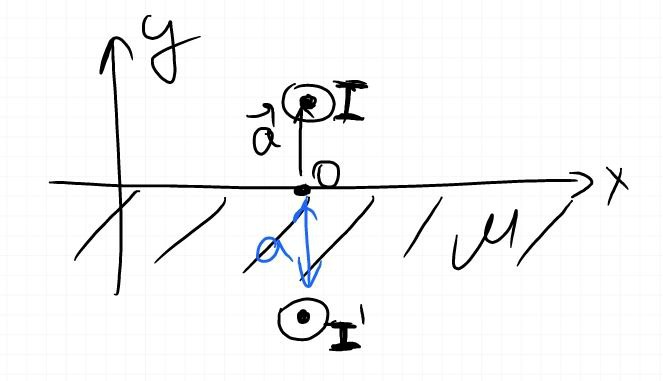
\includegraphics[width=1\textwidth]{photo_1.jpg}
%\par
%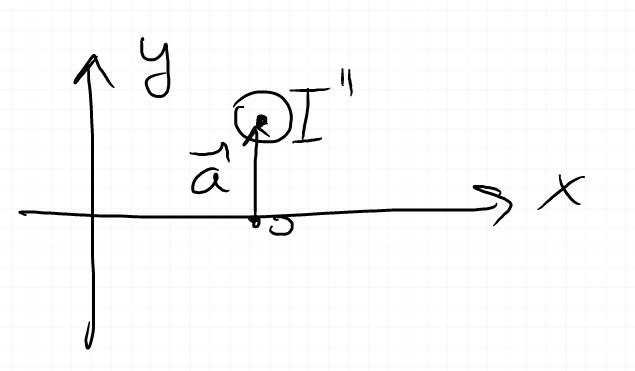
\includegraphics[width=1\textwidth]{photo_2.jpg}
\par
\[
    \overrightarrow{B} = \overrightarrow{B_0} + \overrightarrow{B_1} e^{-i\omega t}
\]
\[
    \overrightarrow{M} = \overrightarrow{M_0} + \overrightarrow{M_1} e^{-i\omega t}
\]
\begin{eqnarray*}
%    \nonumber
    \frac{d\left(  \overrightarrow{M_0} + \overrightarrow{M_1} e^{-i\omega t}\right)}{dt} = \gamma \cdot \left( \overrightarrow{B_0} + \overrightarrow{B_1} e^{-i\omega t} \right) \times \left( \overrightarrow{M_0} + \overrightarrow{M_1} e^{-i\omega t} \right) - \\
    - \frac{\left( \overrightarrow{M_0} + \overrightarrow{M_1} e^{-i\omega t} \right)_{||} - \overrightarrow{M_0}}{T_1} - \frac{\left( \overrightarrow{M_0} + \overrightarrow{M_1} e^{-i\omega t} \right)_{\perp}}{T_2}
\end{eqnarray*}
\[
   -i\omega \overrightarrow{M_1} = \gamma \cdot \left( \overrightarrow{B_0} \times \overrightarrow{M_1} +  \overrightarrow{B_1} \times \overrightarrow{M_0} + \overrightarrow{B_1} \times \overrightarrow{M_1} \right) - \frac{\overrightarrow{M_{1 ||}}}{T_1} - \frac{\overrightarrow{M_{1 \perp}}}{T_1}
\]
\par Слагаемое $\overrightarrow{B_1} \times \overrightarrow{M_1} = 0$, так как это следующий порядок малости:
\[
   -i\omega \overrightarrow{M_1} = \gamma \cdot \left( \overrightarrow{B_0} \times \overrightarrow{M_1} +  \overrightarrow{B_1} \times \overrightarrow{M_0} \right) - \frac{\overrightarrow{M_{1 ||}}}{T_1} - \frac{\overrightarrow{M_{1 \perp}}}{T_1}
\]
\par Считаем что поле по z не меняется в силу малости поля $\overrightarrow{B_1}$ и $M_z = M_0$
\par Проецируем на оси x и y и получаем систему уравнений
\begin{equation*}
    \begin{cases}
        -i\omega M_{1x} = \gamma \left( -B_{0} M_1{1y} + B_{1y} M_1{0} \right) -\frac{M_{1x}}{T_2} \\
        -i\omega M_{1y} = \gamma \left( B_{0} M_1{1x} - B_{1x} M_1{0} \right) -\frac{M_{1y}}{T_2}
    \end{cases}
\end{equation*}
\par В матричном виде получаем уравнение
\begin{equation*}
    \begin{pmatrix}
        \left( 1 -i\omega T_2 \right) & \gamma B_0 T_2 \\
         \gamma B_0 T_2 & - \left( 1 -i\omega T_2 \right) \\
    \end{pmatrix}
    \cdot
    \begin{pmatrix}
        M_{1x} \\
        M_{1y}
    \end{pmatrix}
    = \gamma B_0 T_2 \chi_M
    \begin{pmatrix}
        B_{1y} \\
        B_{1x}
    \end{pmatrix}
\end{equation*}

\begin{equation*}
    \begin{pmatrix}
        M_{1x} \\
        M_{1y}
    \end{pmatrix}
    = \gamma B_0 T_2 \chi_M \cdot
    \begin{pmatrix}
        \left( 1 -i\omega T_2 \right) & \gamma B_0 T_2 \\
         \gamma B_0 T_2 & - \left( 1 -i\omega T_2 \right) \\
    \end{pmatrix}^{-1}
    \begin{pmatrix}
        B_{1y} \\
        B_{1x}
    \end{pmatrix}
\end{equation*}

\begin{equation*}
    \begin{pmatrix}
        M_{1x} \\
        M_{1y}
    \end{pmatrix}
    = \gamma B_0 T_2 \chi_M \frac{1}{\left( 1 -i\omega T_2 \right)^2 + \left( \gamma B_0 T_2 \right)^2} \cdot
    \begin{pmatrix}
        \left( 1 -i\omega T_2 \right) & \gamma B_0 T_2 \\
         \gamma B_0 T_2 & - \left( 1 -i\omega T_2 \right) \\
    \end{pmatrix}
    \begin{pmatrix}
        B_{1y} \\
        B_{1x}
    \end{pmatrix}
\end{equation*}

\begin{equation*}
    \begin{pmatrix}
        M_{1x} \\
        M_{1y}
    \end{pmatrix}
    = \gamma B_0 T_2 \chi_M \frac{1}{\left( 1 -i\omega T_2 \right)^2 + \left( \gamma B_0 T_2 \right)^2} \cdot
    \begin{pmatrix}
         \gamma B_0 T_2 & \left( 1 -i\omega T_2 \right)\\
         - \left( 1 -i\omega T_2 \right) & \gamma B_0 T_2 \\
    \end{pmatrix}
    \begin{pmatrix}
        B_{1x} \\
        B_{1y}
    \end{pmatrix}
\end{equation*}
\par Очевидно что $\chi_{zz} = \chi_M$ в силу линейности поля $B$, а $\chi_{zx} = \chi_{zy} = \chi_{xz} = \chi_{yz} = 0$
\par Графики:
\par $\chi_{xx} = -\chi_{yy}$
\par
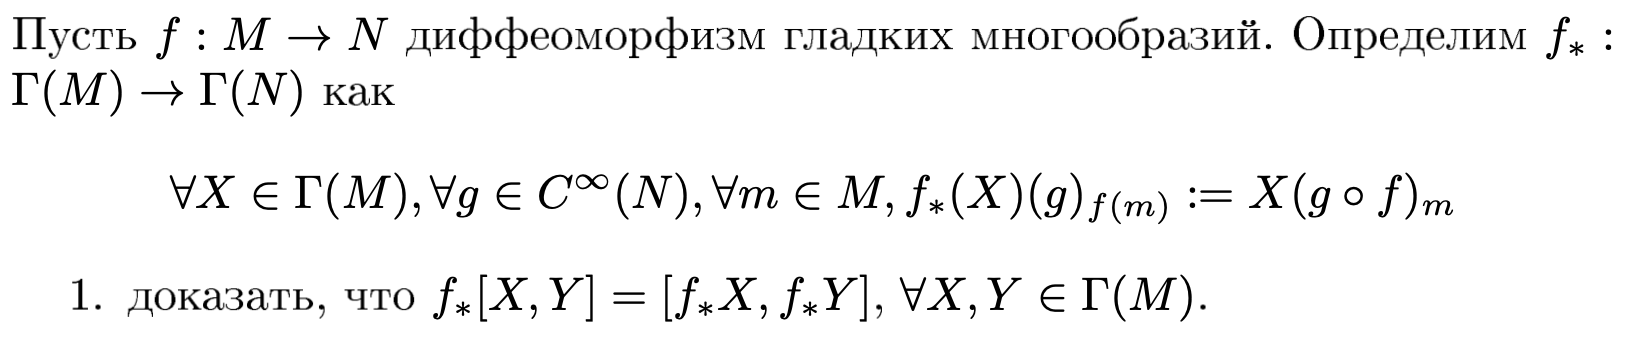
\includegraphics[width=1\textwidth]{photo_1.png}
\par $\chi_{xy} = \chi_{yx}$
\par
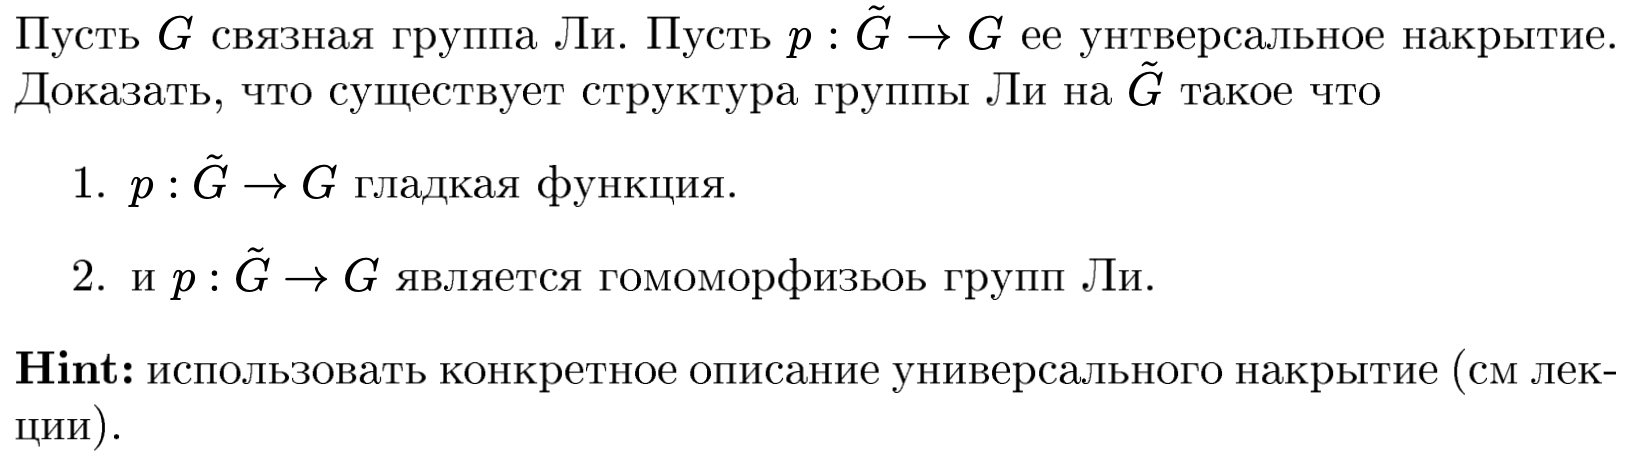
\includegraphics[width=1\textwidth]{photo_2.png}
\end{large}
\end{document}
